% !TEX program = xelatex
\documentclass[UTF8,a4paper,11pt]{ctexart}
\usepackage{amsmath,amssymb}
\usepackage{booktabs}
\usepackage{graphicx}
\usepackage{hyperref}
\usepackage{geometry}
\usepackage{setspace}
\geometry{margin=2.4cm}

% 符号（第 3 节首次定义后全文统一使用）
\newcommand{\Lt}{\mathcal{L}^{\mathrm{tok}}}
\newcommand{\Lti}[1]{\Lt_{#1}}
\newcommand{\slope}{\Delta\Lt}

\title{PRML 作业四：Transformer 复现与模块消融}
\author{黄馨琰 \\ \small \texttt{2495657518@qq.com}}
\date{\today}

\begin{document}
\onehalfspacing
\maketitle

\begin{abstract}
在 Multi30k 德英翻译任务上实现了 Vaswani 等提出的 Encoder--Decoder Transformer，
并完成全量数据下的基线训练与两项模块消融。
基线模型验证集 BLEU 最高约 18.7；去掉子层残差后，前四个 epoch 的训练损失几乎不降、BLEU 接近 0。
位置编码方面，在\textbf{相同}的半量训练数据设定下做了 sin PE 与无 PE 的配对对照：5 个 epoch 后两组 $\Lt$ 均明显下降，但验证 BLEU 上无 PE 组（约 12.7）略高于 sin PE 组（约 10.8），未见正弦 PE 带来稳定增益。
\end{abstract}

\section{引言}

作业要求复现 \emph{Attention Is All You Need}，并通过对照实验弄清各模块是否“真的有用”。
我实现了一个德$\to$英的 seq2seq Transformer，主要做了两件事：全数据跑通基线；在算力允许范围内做残差（2.3）和位置编码（2.1）的消融。

第一次写位置编码部分时，我把“半数据、无位置编码”的曲线和“全数据、有位置编码”的基线画在同一张图上——事后看这是不对的：
数据量减半本身就会让收敛变慢，没法单独归因到“去掉 PE”。返修后补跑了\textbf{半数据 + 有位置编码}（A 组）与\textbf{半数据 + 无 PE}（B 组），只改 PE 这一项再比（见表~\ref{tab:pe_paired}）。

\section{Transformer 复现}

\subsection{模型}

结构按论文：6 层 Encoder、6 层 Decoder；每层有自注意力（Decoder 还有交叉注意力）和两层 FFN；
子层输出与输入残差相加后做 LayerNorm。注意力为
\begin{equation}
  \mathrm{Attention}(Q,K,V)=\mathrm{softmax}\!\left(\frac{QK^\top}{\sqrt{d_k}}\right)V .
\end{equation}
词嵌入上叠加正弦位置编码。模型宽度 512、8 头、FFN 维度 2048，dropout 0.1。

\subsection{数据与训练}

数据来自 Multi30k 德英句对（约 2.9 万训练句）。分词用 spacy；按词频建表；句子截断到 128 token。
优化用 Adam + Noam 学习率（warmup 4000 步）；损失为带 0.1 label smoothing 的交叉熵。
验证、测试用贪心解码，BLEU 分别在 300、500 句上算（不是全集，数值会偏小一些）。

\subsection{基线结果}

全量数据训练 15 个 epoch。验证 BLEU 在 epoch 6、8 附近最高（约 18.7）；训练到后面 loss 又涨上去、BLEU 掉下去——像是过拟合，也可能是学习率后期不太合适。
写报告时我取\textbf{验证 BLEU 最好的那一轮}，不用最后一轮。摘要见表~\ref{tab:baseline}。

\begin{table}[htbp]
  \centering
  \caption{全量基线（正弦位置编码 + 残差）部分 epoch 记录}
  \label{tab:baseline}
  \begin{tabular}{cccc}
    \toprule
    Epoch $i$ & $\Lti{i}$ & valid BLEU ($\times 100$) & 说明 \\
    \midrule
    1 & 5.4213 & 0.17 &  \\
    4 & 2.6380 & 11.47 &  \\
    6 & 2.2061 & \textbf{18.68} & 验证最优附近 \\
    8 & 1.9561 & \textbf{18.62} &  \\
    15 & 2.0040 & 10.28 & 末轮，已变差 \\
    \bottomrule
  \end{tabular}
\end{table}

\section{实验设置与符号}

\paragraph{哪些一样、哪些不一样。}
原先写「消融与基线层数、宽度、优化器、batch size 相同」指的是\textbf{模型结构}和\textbf{优化超参}一致（见表~\ref{tab:config}）；
并不是说每次实验的数据量、训练轮数、早停策略都一样。
残差消融在全量 29000 句上只改「有没有 $x+$ 残差」；位置编码消融在半数据（每 epoch 随机 50\% 句）上只改「有没有 sin PE」。

\begin{table}[htbp]
  \centering
  \caption{各次实验配置对照（$\checkmark$=与全量基线相同）}
  \label{tab:config}
  \small
  \begin{tabular}{lccc}
    \toprule
    项目 & 全量基线 & 2.3 无残差 & 2.1 半数据 A/B \\
    \midrule
    6 层 / $d{=}512$ / 8 头 / FFN 2048 & $\checkmark$ & $\checkmark$ & $\checkmark$ \\
    Adam + Noam（warmup 4000）& $\checkmark$ & $\checkmark$ & $\checkmark$ \\
    batch size 128，label smoothing 0.1 & $\checkmark$ & $\checkmark$ & $\checkmark$ \\
    训练句数 / epoch & 29000 & 29000 & 14500（50\%） \\
    计划 epoch 数 & 15 & 5 & 5 \\
    早停 & 无（跑满） & patience$=3$ & 关闭 \\
  \midrule
    \textbf{单变量改动} & --- & 关残差 & A：sin PE；B：无 PE \\
    \bottomrule
  \end{tabular}
\end{table}

\paragraph{符号表示}
设第 $i$ 个训练 epoch 结束后的\textbf{平均每 token 交叉熵}为 $\Lti{i}$（即日志里的 train loss/token）。
验证集 BLEU 记为 $B_i$（表中有时写成百分数，即 $100\times B_i$）。
前四个 epoch 的损失下降“斜率”定义为
\begin{equation}
  \slope \;=\; \frac{\Lti{1}-\Lti{4}}{4},
  \label{eq:slope}
\end{equation}
表示这 4 轮里 loss 平均每 epoch 下降多少；$\slope$ 越大，前期收敛越快。

\paragraph{半数据模式}
算力不够跑全量消融时，采用\textbf{半数据模式}：固定随机种子，每个 epoch 只随机用 50\% 的训练句（约 14500 句），共训练 5 个 epoch，不早停。
位置编码对比\textbf{必须}在半数据模式下比较两条曲线：一条保留正弦 PE，一条去掉 PE；其它设置相同。全量基线只用来展示“模型能训起来”，不参与 PE 的同级对比。

\section{残差消融（2.3）}

\subsection{实验设置}

唯一改动：关闭 Encoder/Decoder 子层里的 $x+\mathrm{Sublayer}(x)$，改成只做 $\mathrm{LayerNorm}(\mathrm{Sublayer}(x))$。
位置编码、数据量、层数与全量基线一致（全量 29000 句，训练 5 epoch，第 4 epoch 后早停）。

\subsection{结果}

表~\ref{tab:ablation} 是前 4 个 epoch 的 $\Lt$ 和 $B_4$。图~\ref{fig:ablation_23} 为同一数据的曲线。

\begin{table}[htbp]
  \centering
  \caption{有残差（全量基线）与无残差（全量）前四 epoch 对比}
  \label{tab:ablation}
  \begin{tabular}{lcccccc}
    \toprule
    设置 & $\Lti{1}$ & $\Lti{2}$ & $\Lti{3}$ & $\Lti{4}$ & $100\cdot B_4$ & $\slope$ \\
    \midrule
    有残差 & 5.4213 & 3.6305 & 2.9902 & 2.6380 & 11.47 & 0.6958 \\
    无残差 & 5.6614 & 4.5614 & 4.4089 & 4.3282 & 0.0024 & 0.3333 \\
    \bottomrule
  \end{tabular}
\end{table}

\begin{figure}[htbp]
  \centering
  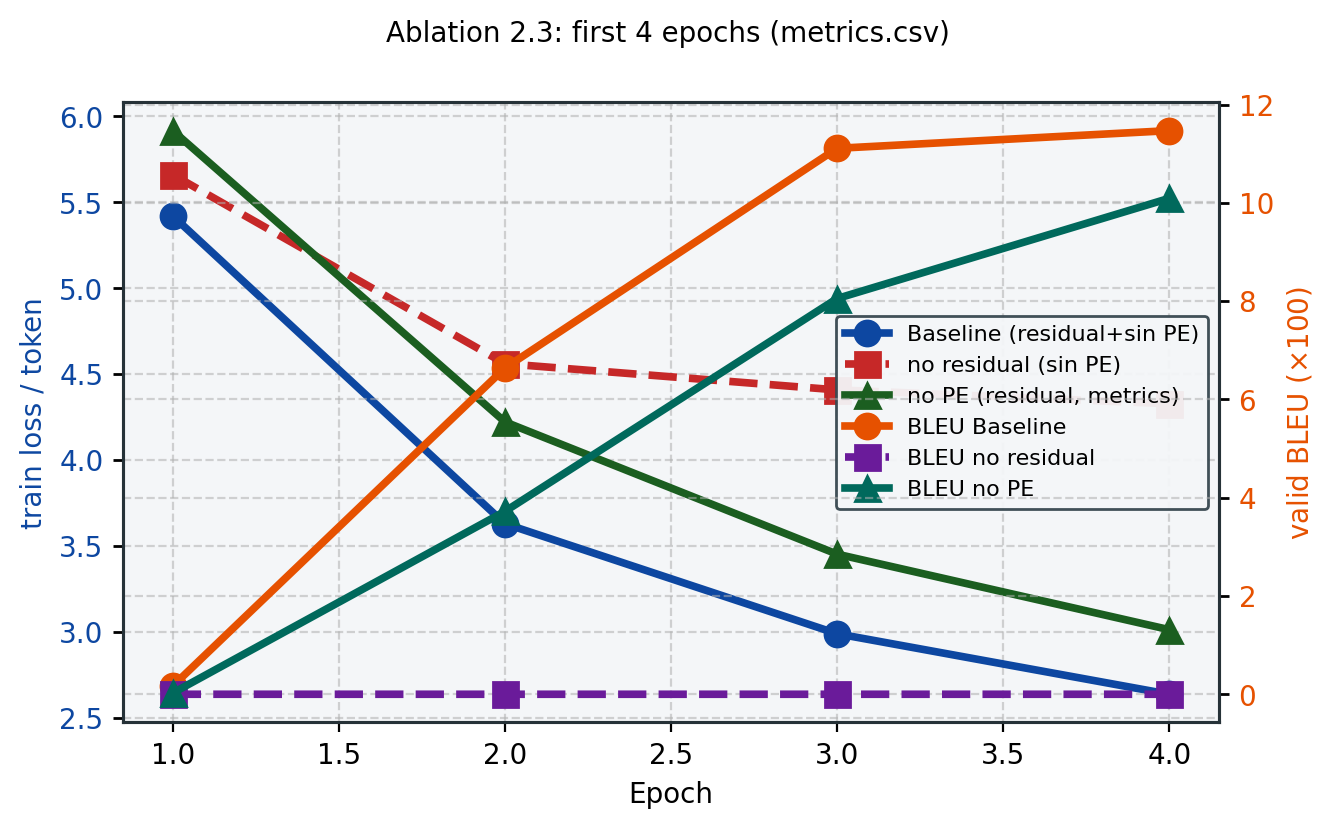
\includegraphics[width=0.92\textwidth]{report/fig_ablation_2_3_ep1_4.png}
  \caption{残差消融：前 4 epoch 的训练损失与验证 BLEU}
  \label{fig:ablation_23}
\end{figure}

\subsection{讨论}

有残差时，第一轮 $\Lti{1}\approx 5.42$，四轮下来 $\slope\approx 0.70$，$B_4$ 能到 11 左右。
无残差时，第一轮 loss 就更高（5.66），四轮后还在 4.33 附近晃，$B_4$ 基本是 0——译出来的东西和乱猜差不多。
第 4 epoch 后验证 BLEU 一直起不来，触发了早停。

我自己的理解（不一定严谨）：6 层堆在一起，如果没有那条“直接把输入加回去”的路，每一层都得靠训练去模仿恒等映射，前期梯度很难传下去，所以 loss 掉得极慢。
论文里 ResNet 那套说法在这里能对上号，但对我更有用的是表里的数：\textbf{关掉残差，这个规模的模型前几轮等于没在学翻译}。

\section{位置编码消融（2.1）}

\subsection{实验设置}

在半数据模式下，对照 A：正弦位置编码 + 残差；对照 B：去掉位置编码（嵌入不再加 PE）+ 残差。
两组都用相同的 50\% 采样方式和 5 个 epoch。此前版本曾把 B 和\textbf{全量}基线画在一起，已作废；正文只保留 A vs B。

\subsection{结果}

无 PE 组（B）的逐 epoch 数据见表~\ref{tab:none_pe}。
有 PE 的对照组（A）与 B 组均在半数据模式下训满 5 个 epoch；逐 epoch 数值见表~\ref{tab:pe_paired}，配对曲线见图~\ref{fig:pe_paired}。

\begin{table}[htbp]
  \centering
  \caption{半数据、无位置编码（B 组）}
  \label{tab:none_pe}
  \begin{tabular}{ccc}
    \toprule
    $i$ & $\Lti{i}$ & $100\cdot B_i$ \\
    \midrule
    1 & 5.9176 & 0.03 \\
    3 & 3.4533 & 8.05 \\
    5 & 2.7098 & 12.72 \\
    \bottomrule
  \end{tabular}
\end{table}

\begin{table}[htbp]
  \centering
  \caption{半数据位置编码对照（A：sin PE；B：无 PE）}
  \label{tab:pe_paired}
  \begin{tabular}{lcc|cc}
    \toprule
    $i$ & \multicolumn{2}{c|}{A：sin PE} & \multicolumn{2}{c}{B：无 PE} \\
        & $\Lti{i}$ & $100\cdot B_i$ & $\Lti{i}$ & $100\cdot B_i$ \\
    \midrule
    1 & 5.8939 & 0.02 & 5.9176 & 0.03 \\
    3 & 3.7045 & 5.34 & 3.4533 & 8.05 \\
    5 & 2.9457 & 10.81 & 2.7098 & 12.72 \\
    \bottomrule
  \end{tabular}
\end{table}

\begin{figure}[htbp]
  \centering
  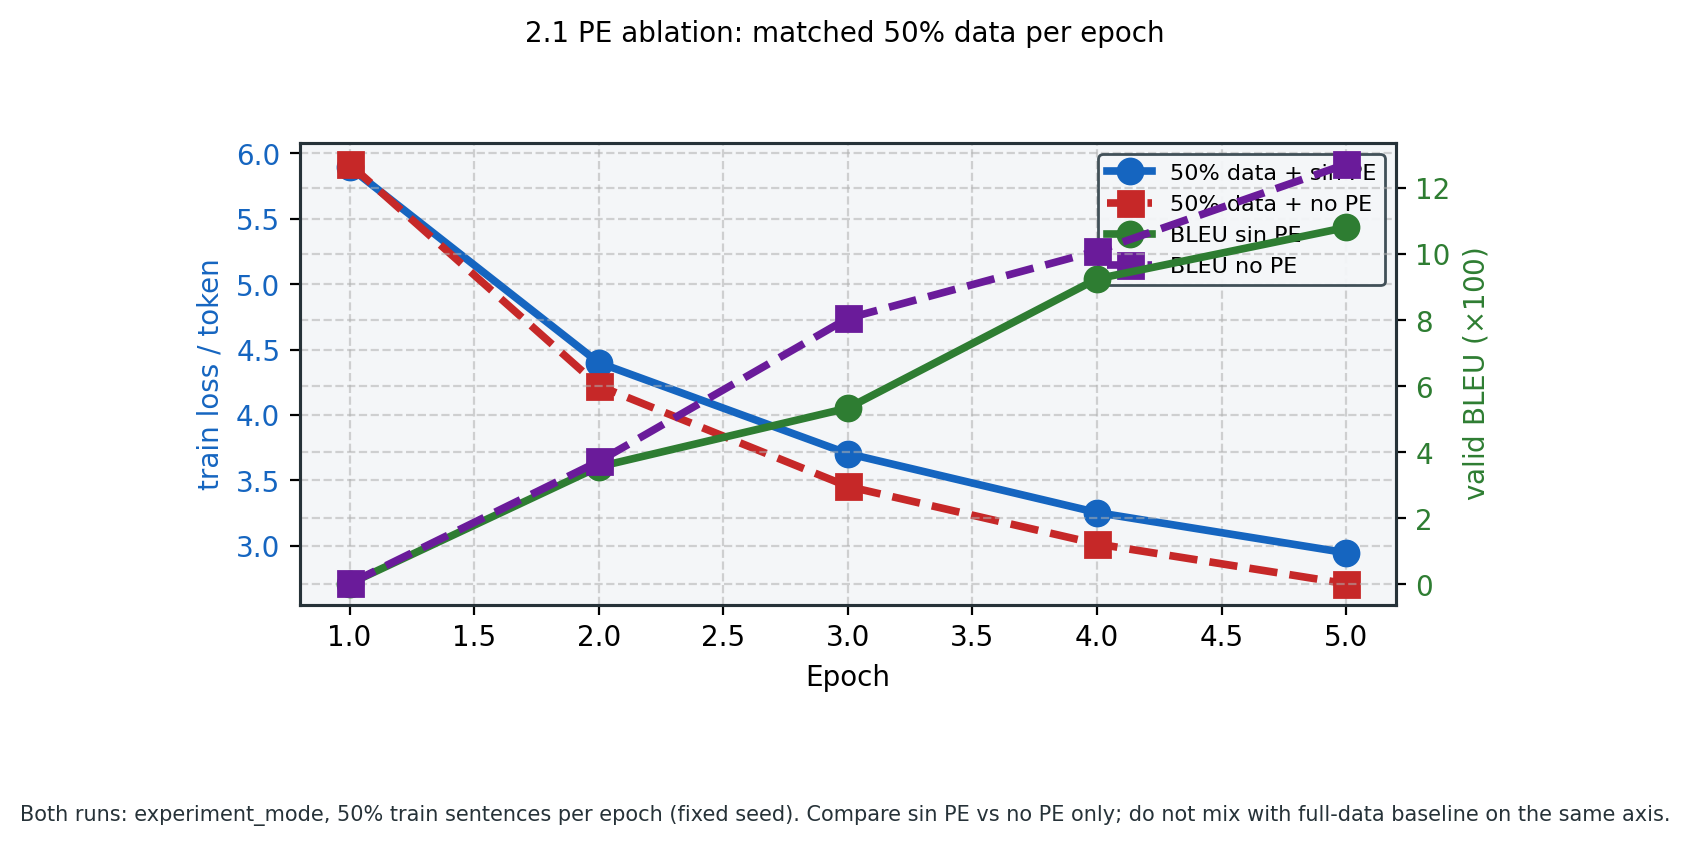
\includegraphics[width=0.88\textwidth]{report/fig_2_1_pe_paired.png}
  \caption{半数据模式下，仅位置编码不同时的 loss 与 BLEU（A：sin PE，B：无 PE）}
  \label{fig:pe_paired}
\end{figure}

\subsection{讨论}

\textbf{无 PE 时模型情况}：无 PE 时模型不是完全训不动，B 组 5 个 epoch 里 loss 从 5.9 降到 2.7，BLEU 也能到 12 左右。
但 Decoder 还有因果 mask，源端也有序列顺序，所以“一点位置信息都没有”并不等于“一点顺序都没有”——能学到一些东西并不奇怪。

\textbf{对比是否公平}：PE 部分只应在表~\ref{tab:config} 里「半数据 A/B」两行之间比；若只拿 B 去和全量基线比，我会分不清是 PE 的锅还是数据变少的锅。
配对结果（表~\ref{tab:pe_paired}）：第 1 epoch 两组 $\Lt_1$ 都在 5.9 附近、$B_1\approx 0$；到第 3 epoch，B 的 $\Lt_3=3.45$、$B_3=8.05$，已略优于 A（$\Lt_3=3.70$，$B_3=5.34$）；第 5 epoch 仍如此——B 的 $\Lt_5=2.71$、$B_5=12.72$，A 为 $\Lt_5=2.95$、$B_5=10.81$。
因此在「半数据 + 5 epoch + 本实现」下，\textbf{不能}说正弦 PE 带来了更高的验证 BLEU；反而无 PE 组略好，可能与随机 50\% 子采样、学习率日程等噪声有关，需要更长训练或多次 seed 才能下更强结论。
推断阶段关掉 PE 时注意力更散（第 7 节热力图）与「训练时完全不加 PE 反而 BLEU 略高」并不矛盾：前者是同一组权重上的推理消融，后者是重新训练得到的另一套参数。

全量基线的训练曲线单独放在第 8 节，\textbf{不}与图~\ref{fig:pe_paired} 混画。

\section{注意力热力图}

图~\ref{fig:attn0}、图~\ref{fig:attn7} 用的是\textbf{全量基线}训练得到的权重（sin PE），在测试集句子上画 Encoder 第 5 层（最后一层）的 8 个头。
左/上为推断时\textbf{保留}位置编码（与训练一致）；右/下为\textbf{同一组权重}、推断时关掉 PE（不重训）。
这不是又训了一个无 PE 模型，只是看「位置表在推理阶段起什么作用」。

测试句 index 0（图~\ref{fig:attn0}）：开 PE 时多个头在对角附近更亮；关 PE 后色块更匀，标题里的 Attention Entropy 会变大（匹配更散）。
index 7（图~\ref{fig:attn7}）更长，现象类似。
色条固定在 $[0,1]$，方便两张图比明暗。推理时必须关掉 Dropout（eval 模式），否则热力图上的斑点是噪声，不能当真。

\begin{figure}[htbp]
  \centering
  \begin{minipage}{0.48\textwidth}
    \centering
    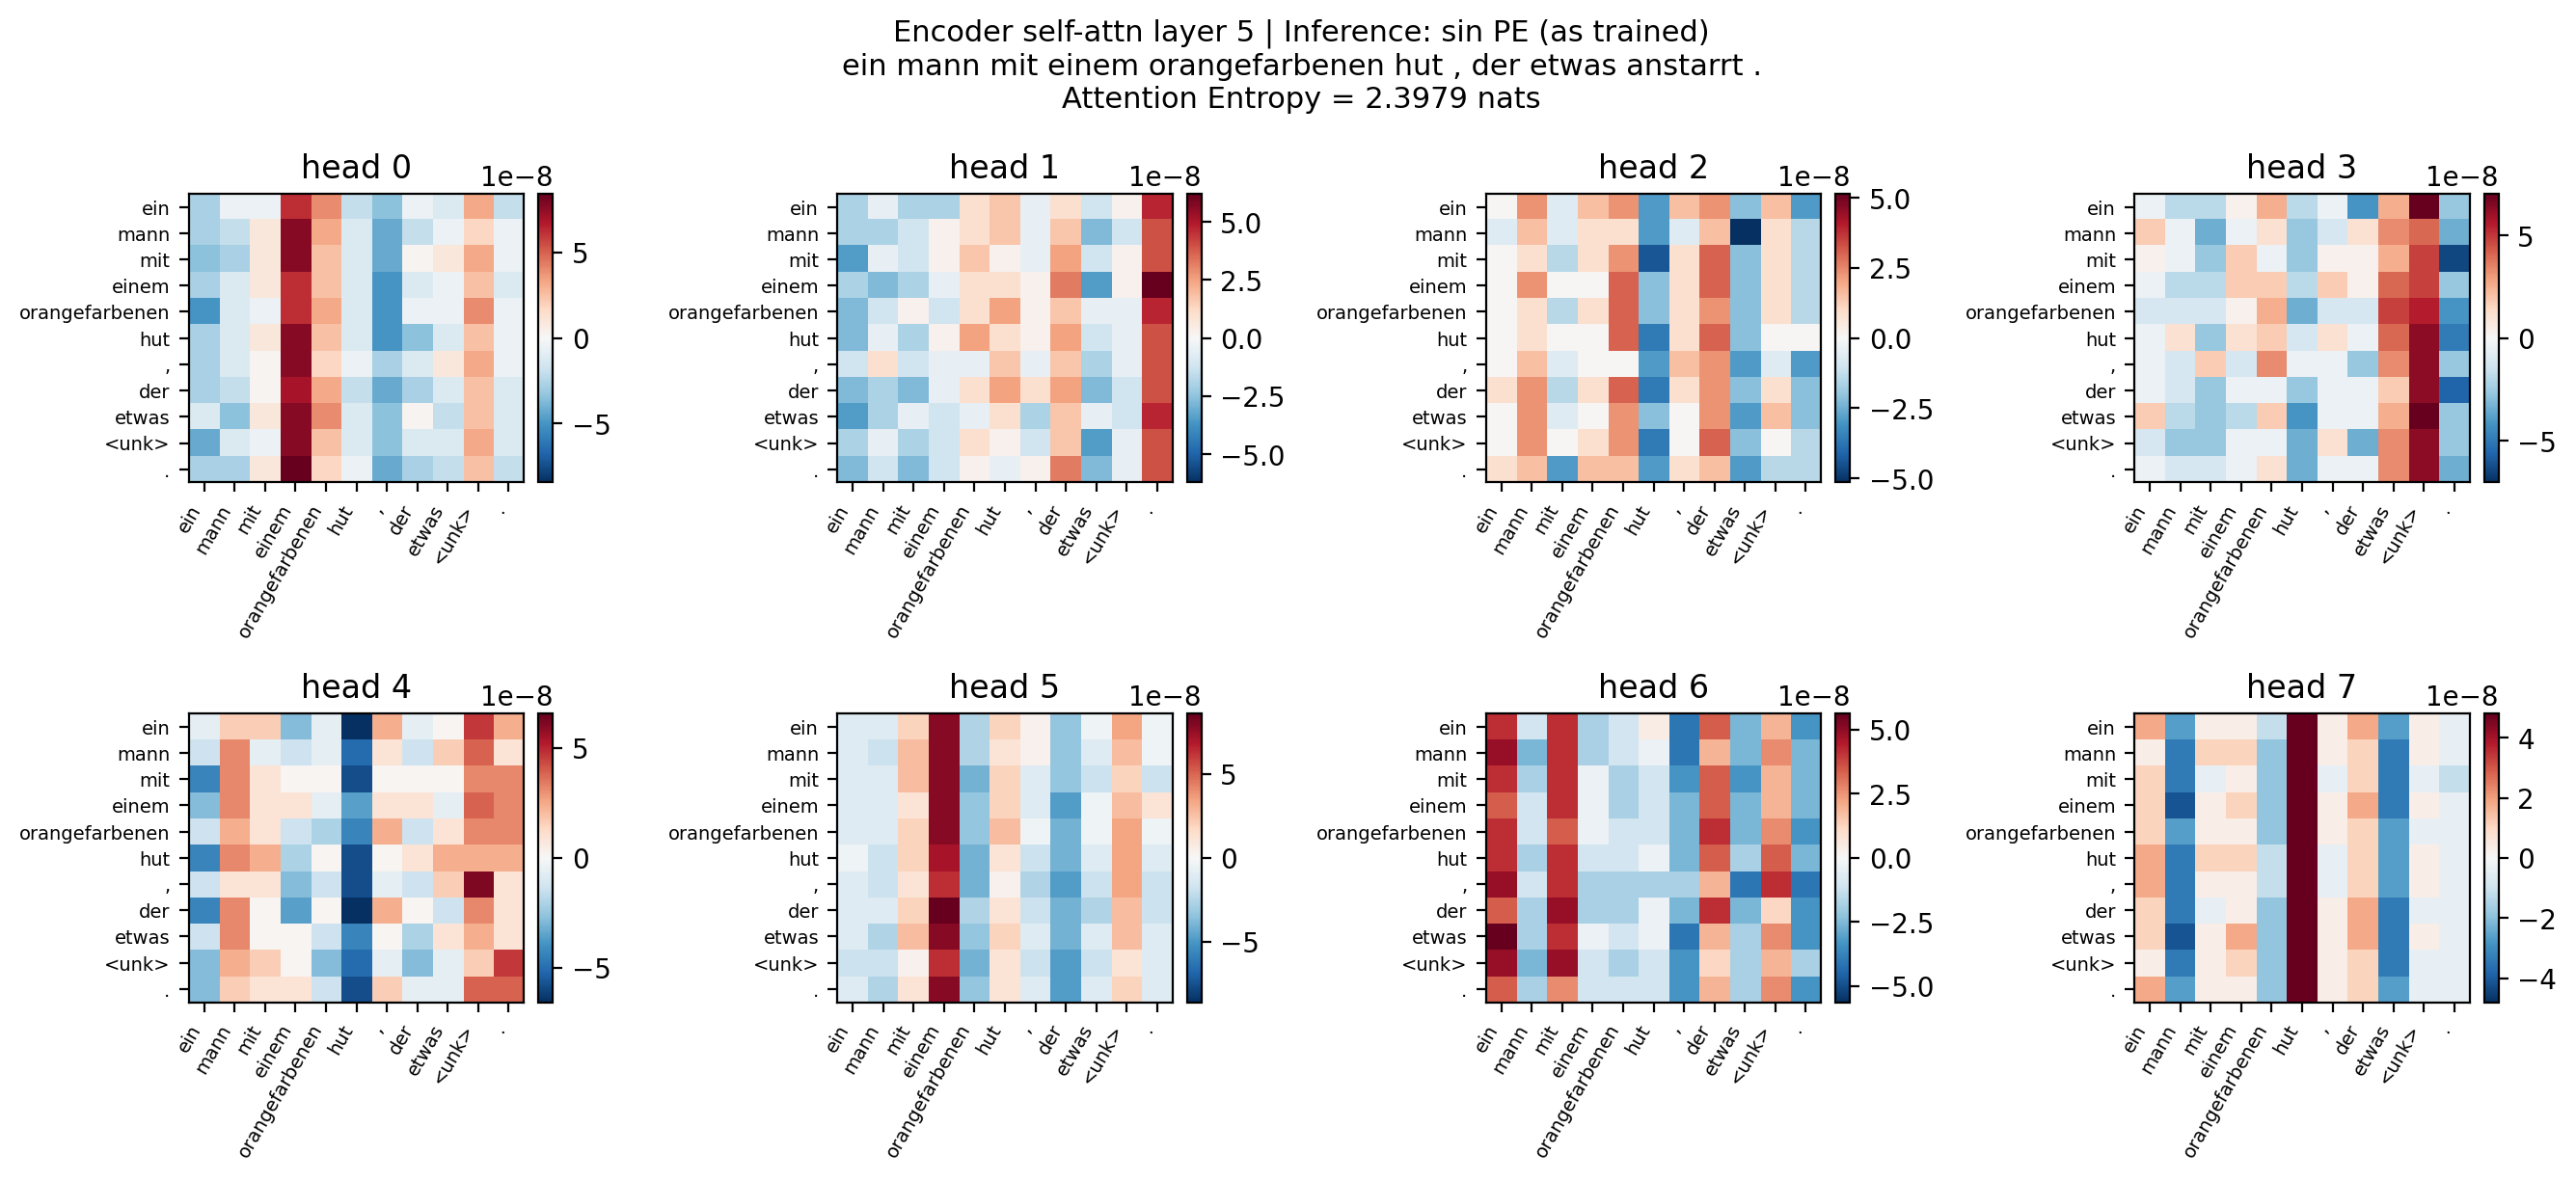
\includegraphics[width=\linewidth]{report/fig_attn_ex0_sin.png}
  \end{minipage}\hfill
  \begin{minipage}{0.48\textwidth}
    \centering
    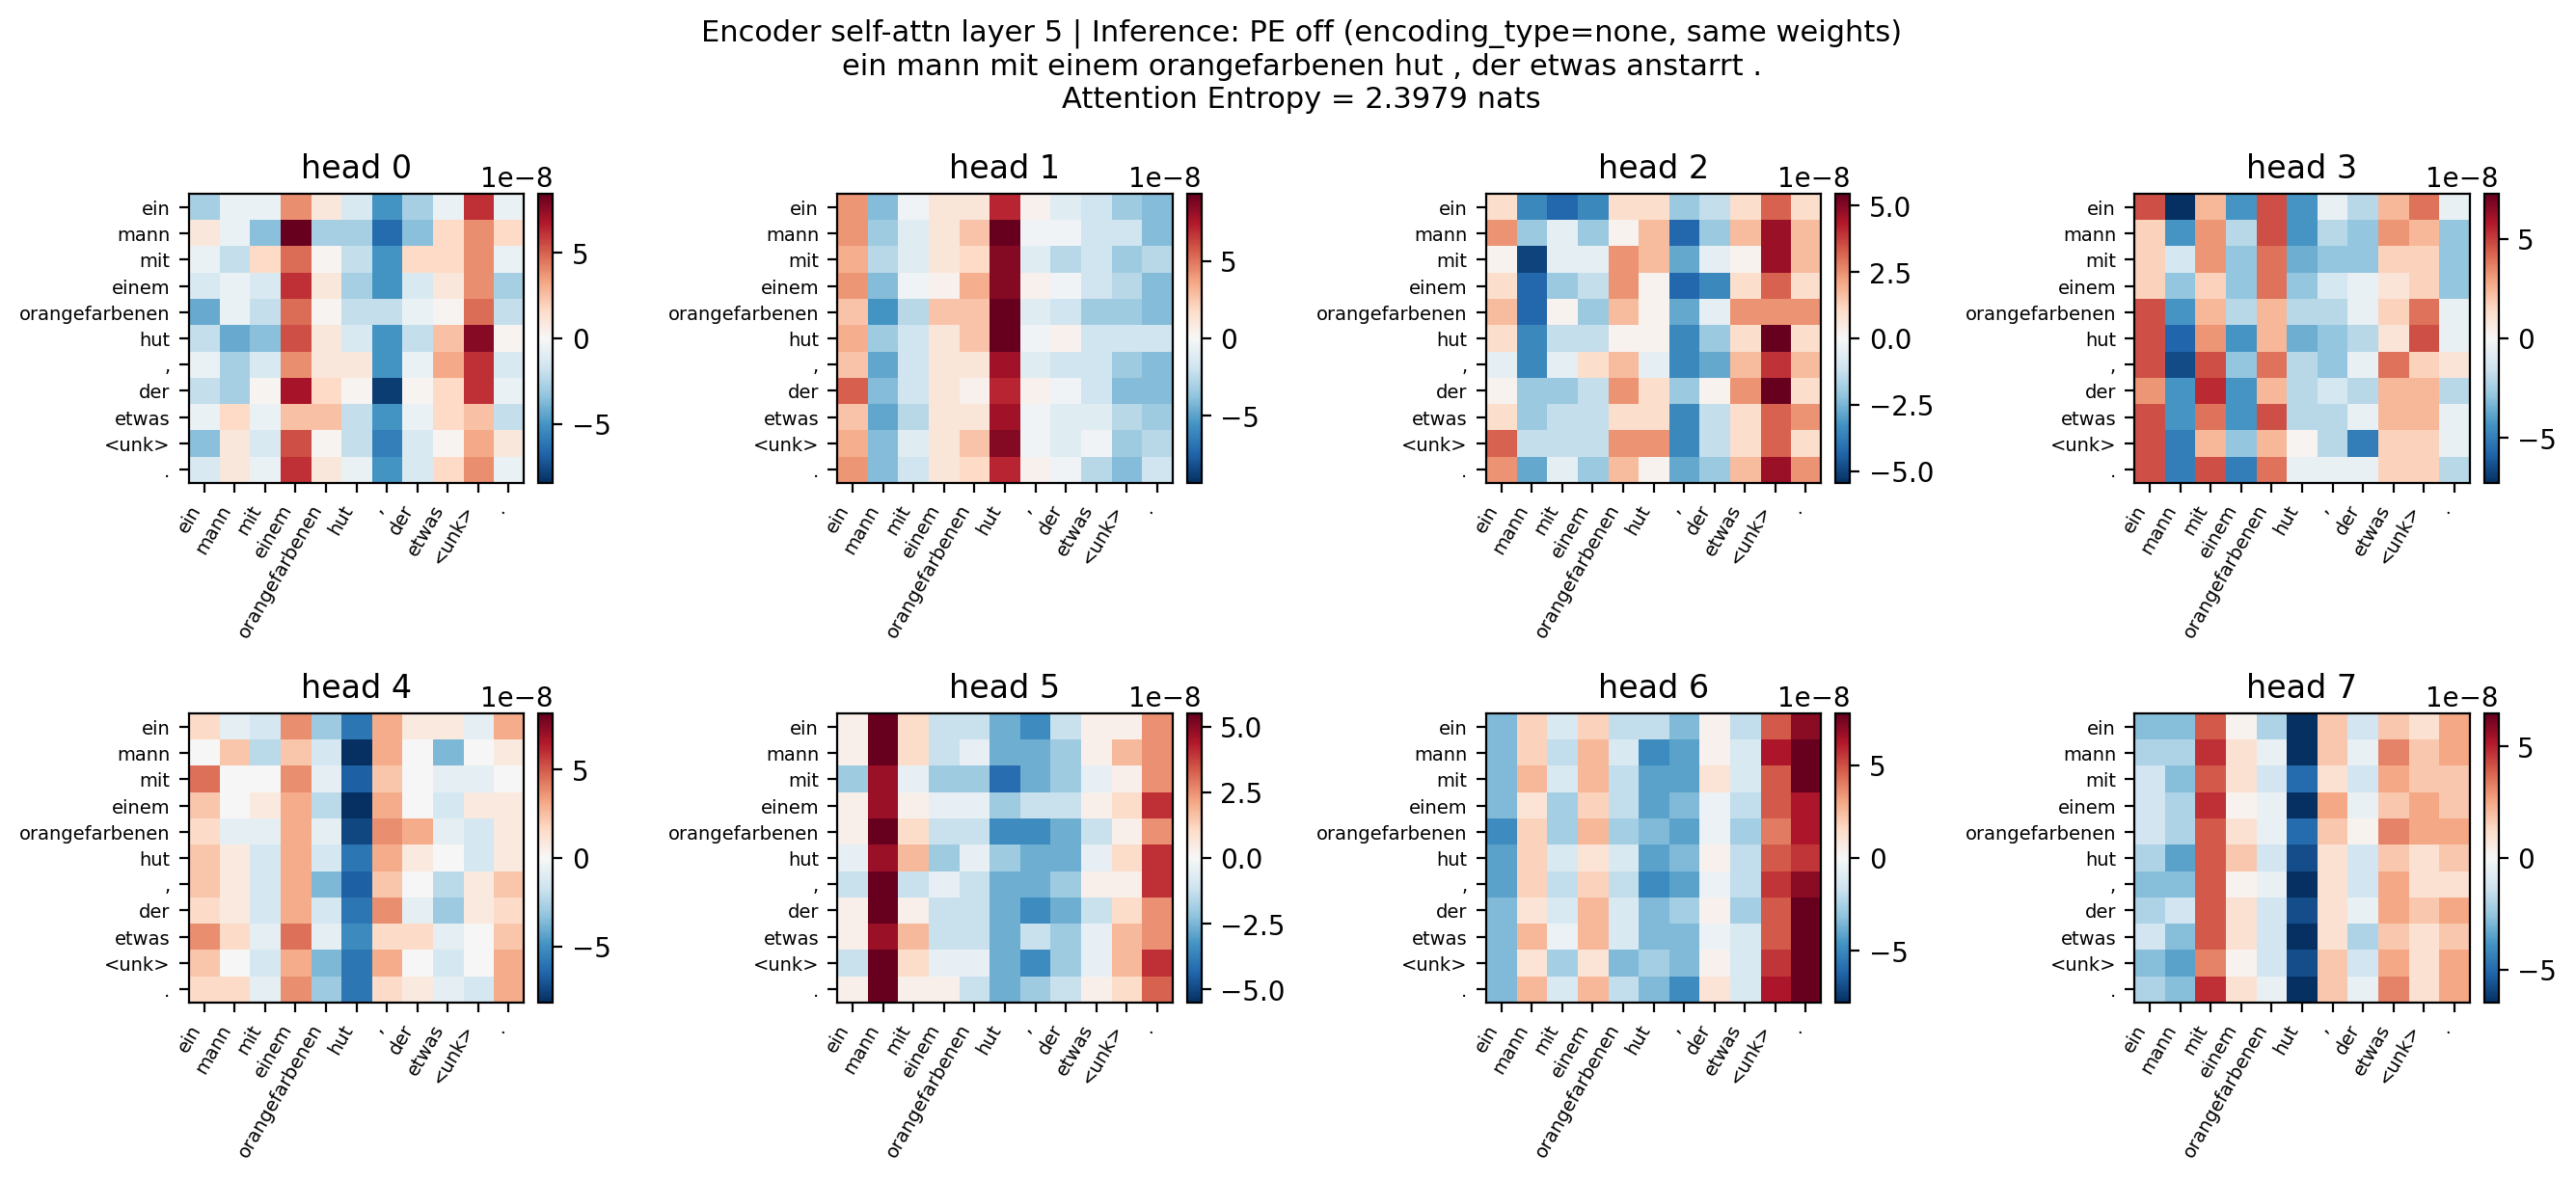
\includegraphics[width=\linewidth]{report/fig_attn_ex0_none.png}
  \end{minipage}
  \caption{测试句 0：sin PE（左）与推断期关 PE（右），Encoder 层 5 多头自注意力}
  \label{fig:attn0}
\end{figure}

\begin{figure}[htbp]
  \centering
  \begin{minipage}{0.48\textwidth}
    \centering
    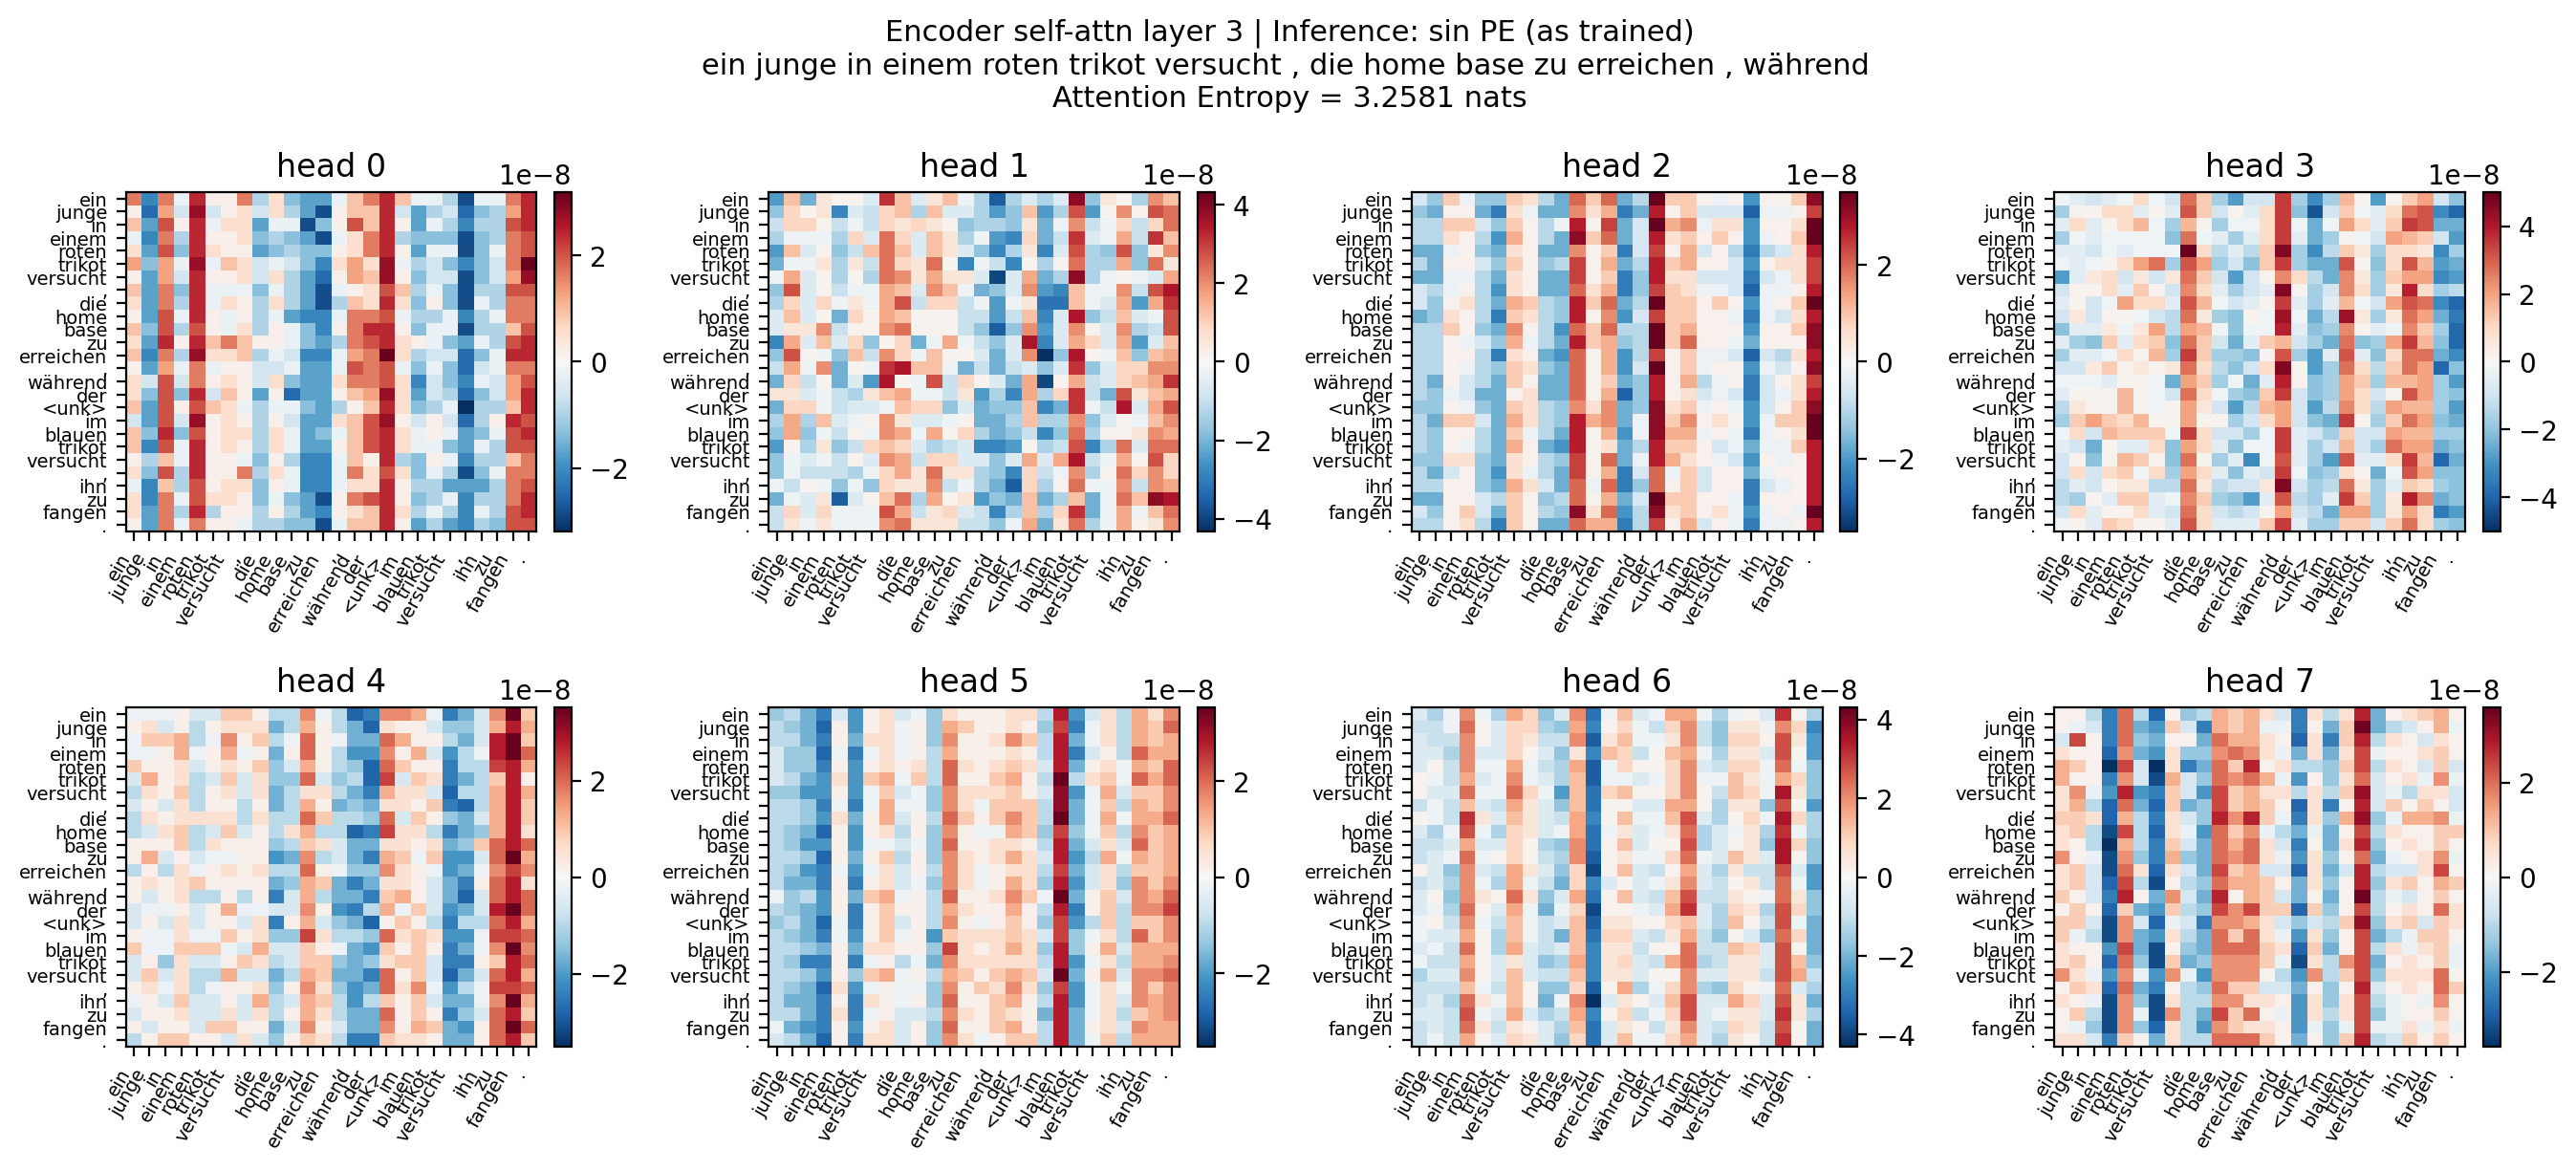
\includegraphics[width=\linewidth]{report/fig_attn_ex7_sin.png}
  \end{minipage}\hfill
  \begin{minipage}{0.48\textwidth}
    \centering
    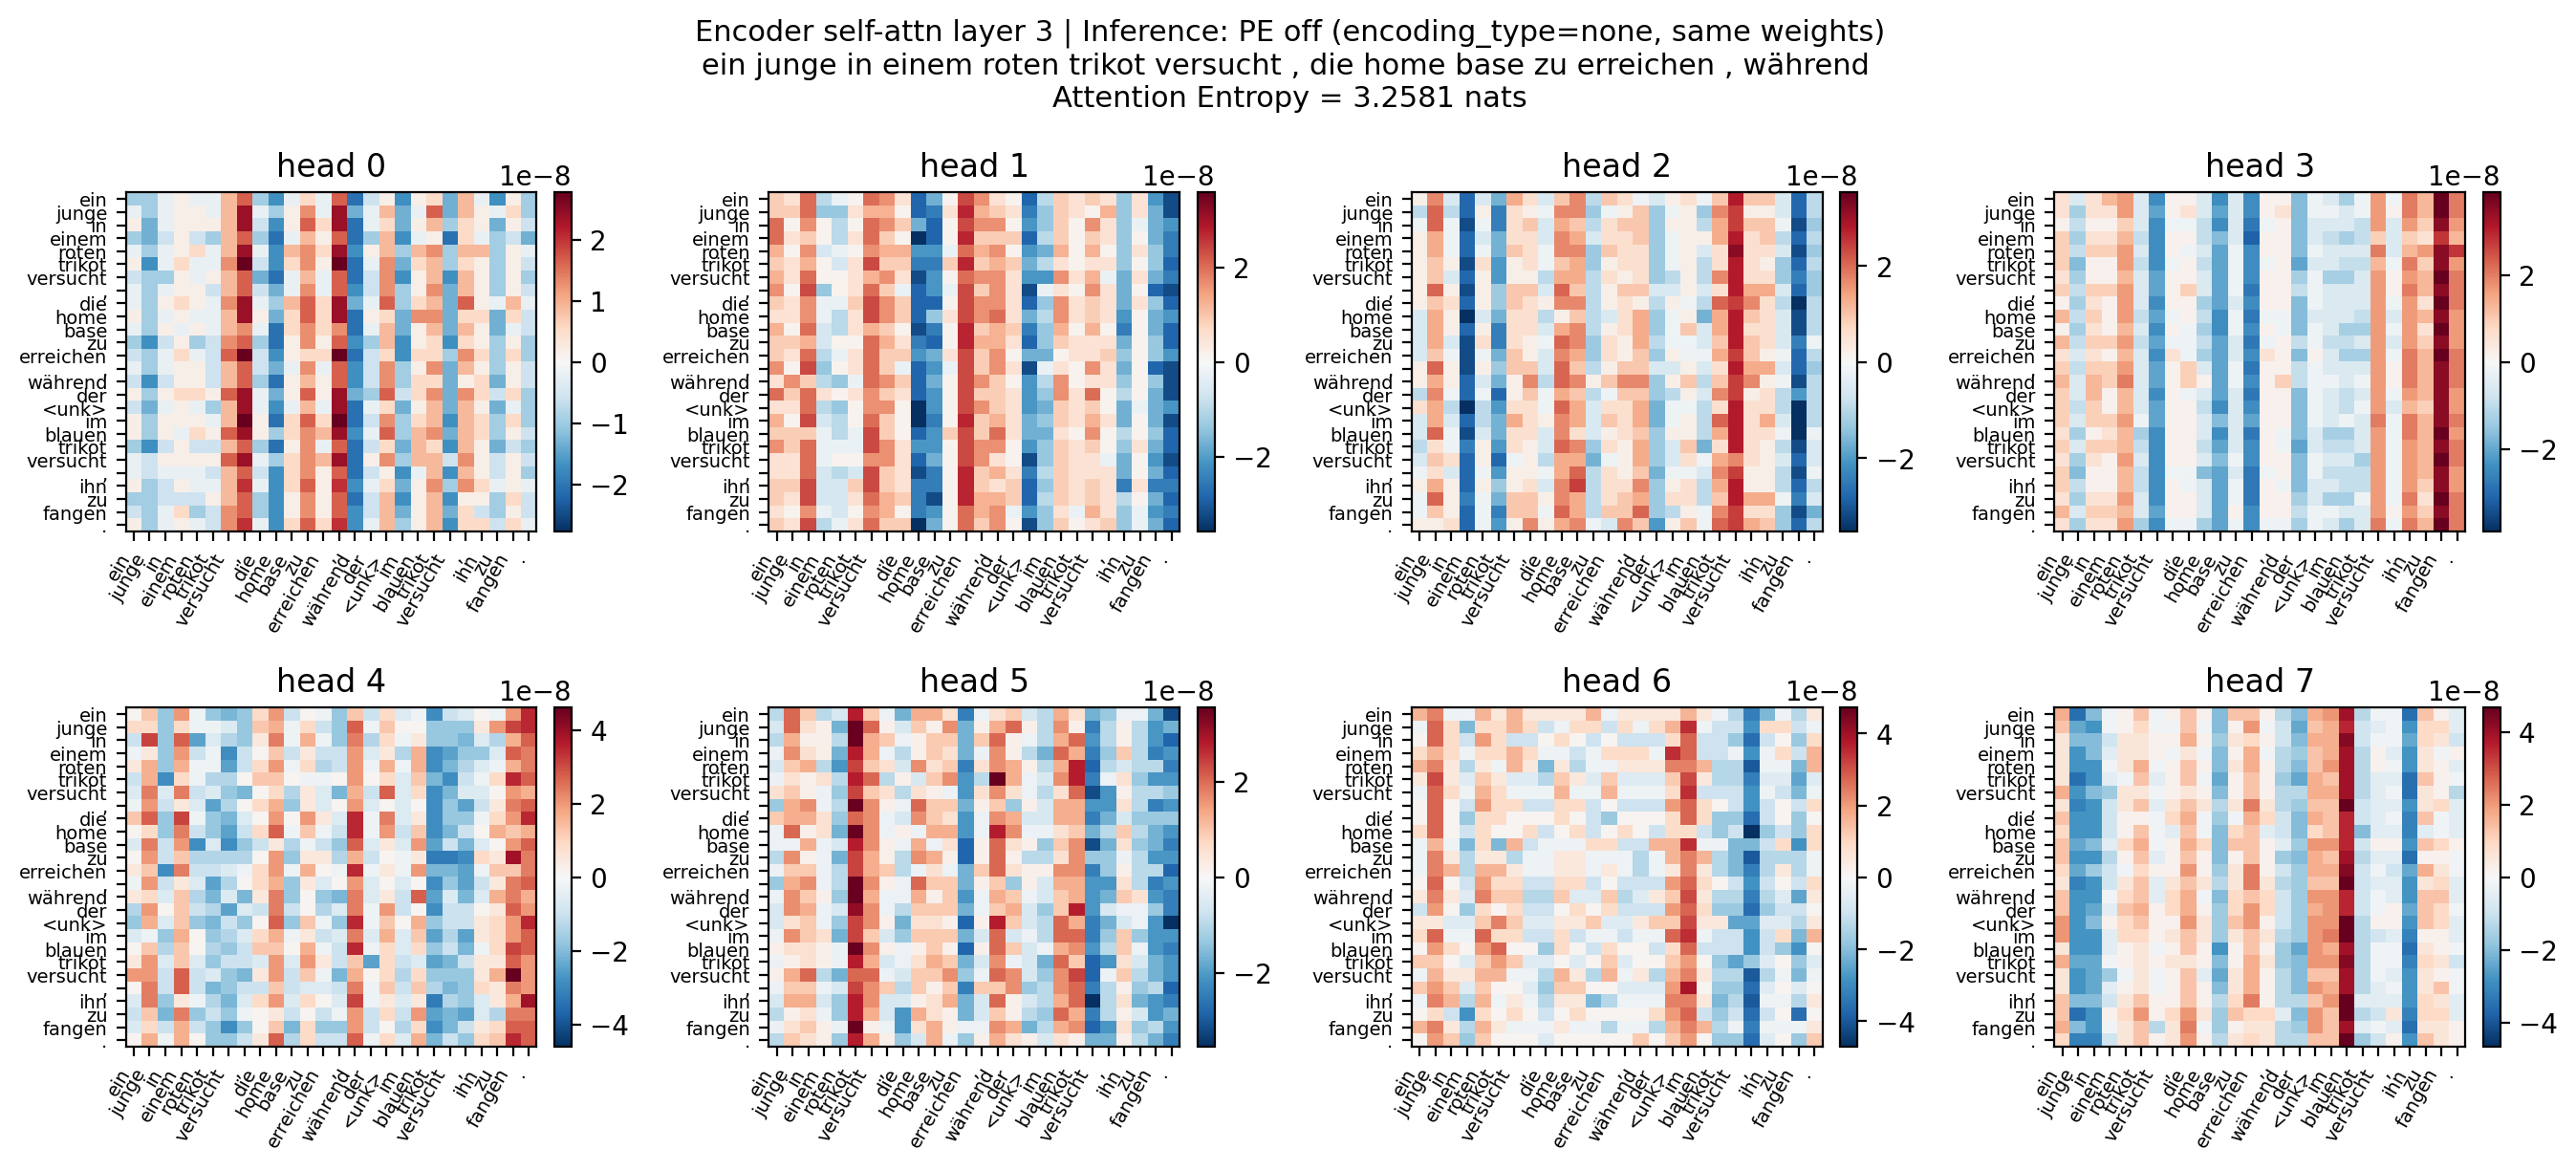
\includegraphics[width=\linewidth]{report/fig_attn_ex7_none.png}
  \end{minipage}
  \caption{测试句 7：同上对比}
  \label{fig:attn7}
\end{figure}

说明：\texttt{report/} 里还有 \texttt{fig\_2\_1\_no\_pe\_loss\_bleu.png}、\texttt{fig\_2\_1\_vs\_baseline\_ref\_early.png} 是返修\textbf{前}用的曲线（半数据无 PE vs 全量基线叠图）；正文已改用表~\ref{tab:pe_paired} 与图~\ref{fig:pe_paired} 的配对设计，故不再插入那两张旧图。

\section{基线训练曲线与 checkpoint}

\begin{figure}[htbp]
  \centering
  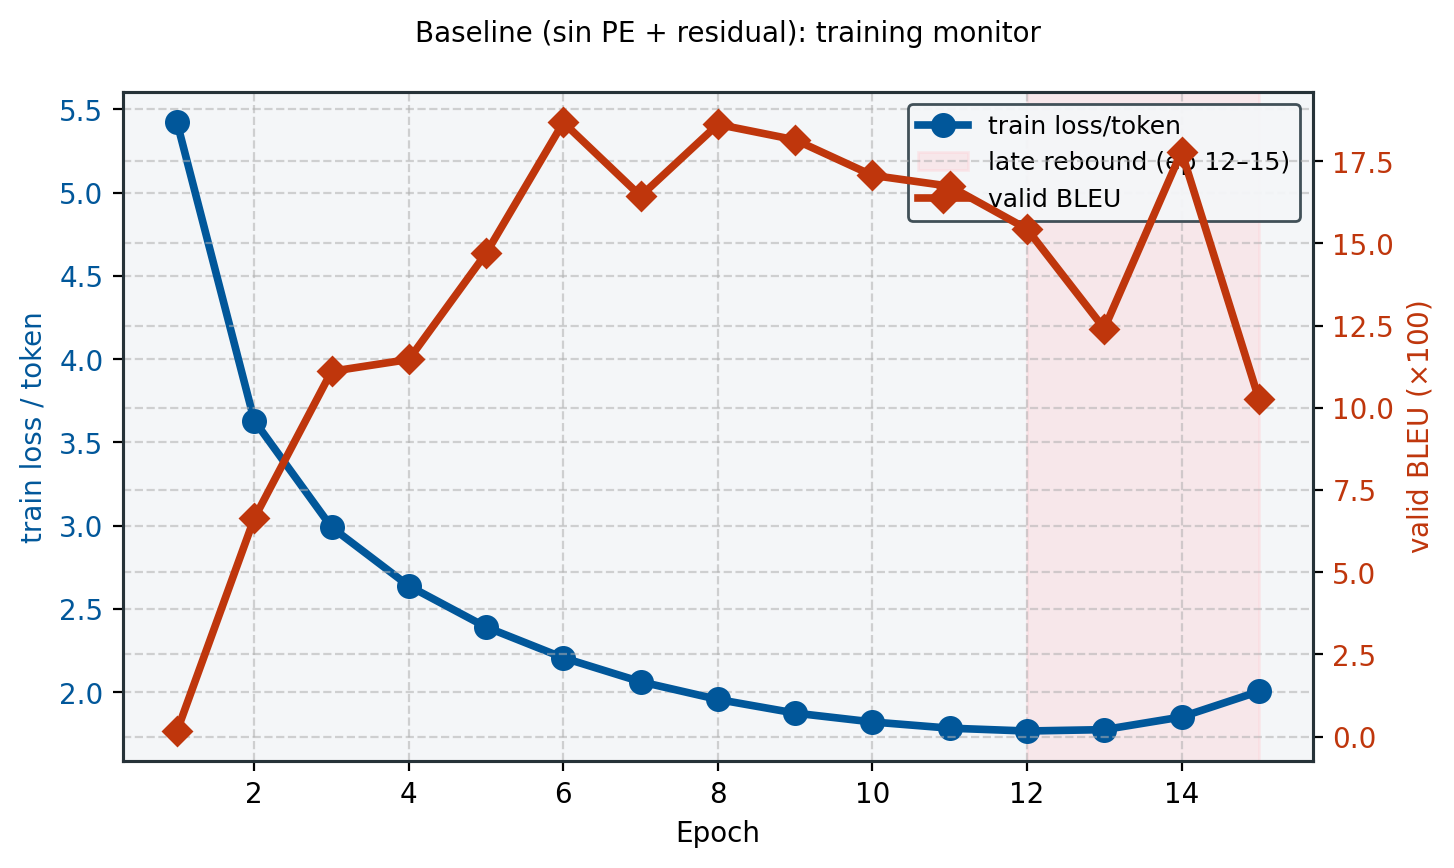
\includegraphics[width=0.92\textwidth]{report/fig_baseline_train_monitor.png}
  \caption{全量基线 15 epoch：$\Lt$ 与验证 BLEU}
  \label{fig:baseline_monitor}
\end{figure}

图~\ref{fig:baseline_monitor} 里，epoch 12 以后训练 loss 反弹、BLEU 下滑。
我后来都存 valid BLEU 最好的权重，不用第 15 轮的。若继续训，可能会加早停，但作业时间里先做到“知道末轮不代表最好”即可。

\section{总结}

\begin{itemize}
  \item 基线能到 valid BLEU $\approx 18.7$，说明实现和训练管线基本可用。
  \item 无残差时前几轮几乎学不到翻译；残差对深层 Transformer 不是可选项，至少在小数据 epoch 数下是这样。
  \item 半数据 PE 配对（表~\ref{tab:pe_paired}）：5 epoch 内无 PE 组 BLEU 略高于 sin PE 组，与“PE 一定提升 BLEU”的直觉不一致；残差消融结论仍明确。
\end{itemize}

\section{附录：复现与工程细节}

\subsection{仓库主要文件}

\begin{itemize}
  \item \texttt{transformer\_model.py}：模型与消融开关（残差、位置编码、QKV 模式）。
  \item \texttt{train.py}：训练、验证、写 \texttt{runs/run\_<时间戳>/}。
  \item \texttt{analyze\_ablation.py}：画消融曲线、生成表格。
  \item \texttt{visualize\_attention.py}：注意力热力图。
\end{itemize}

\subsection{训练命令}

\begin{verbatim}
cd hw_4

# 全量基线
python train.py --local-repo <path>/dataset-master

# 2.3 无残差（全量，config 默认 use_residual=False 或见仓库说明）
python train.py --local-repo <path>/dataset-master

# 2.1 半数据 + 无 PE（B 组，已完成）
python train.py --local-repo <path>/dataset-master --experiment \
  --pos-encoding none --epochs 5 --use-residual --no-early-stopping

# 2.1 半数据 + sin PE（A 组，对照，须与 B 组同 seed / 同 experiment 逻辑）
python train.py --local-repo <path>/dataset-master --experiment \
  --pos-encoding sin --epochs 5 --use-residual --no-early-stopping
\end{verbatim}

B 组：\texttt{report/none\_pe\_experiment\_metrics.csv}（\texttt{runs/run\_1778835536975079123/}）。
A 组：\texttt{report/half\_sin\_pe\_experiment\_metrics.csv}（\texttt{runs/run\_1778917710396986673/}；best valid BLEU $\approx 10.81$，test $\approx 10.88$）。

\subsection{作图命令}

\begin{verbatim}
# 2.3
python analyze_ablation.py --out-fig report/fig_ablation_2_3_ep1_4.png

# 2.1 配对对照（A、B 均半数据）
python analyze_ablation.py \
  --half-sin-pe-csv report/half_sin_pe_experiment_metrics.csv \
  --none-pe-csv report/none_pe_experiment_metrics.csv \
  --out-fig-2-1-paired report/fig_2_1_pe_paired.png --early-epochs 5

# 全量基线监控
python analyze_ablation.py --out-fig-monitor report/fig_baseline_train_monitor.png

# 注意力
python visualize_attention.py --checkpoint runs/<run>/best_model.pt \
  --run-dir runs/<run> --test-index 0 --layer 5 --attn-colorbar fixed01
\end{verbatim}

\subsection{编译}

在 \texttt{hw\_4/} 下执行 \texttt{xelatex hw\_4.tex}。

\end{document}
